\subsection*{Grading Policy}
The typical NC State grading scale will be used. I reserve the right to curve the scale dependent on overall class scores at the end of the semester. Any curve will only ever make it easier to obtain a certain letter grade. The grade will count the assessments using the following proportions:
\begin{itemize}
	\item \underline{\textbf{30\%}} of your grade will be determined by 2 in class midterm exams (15\% each).
	\item \underline{\textbf{5\%}} of your grade will be determined by ...
	\item \underline{\textbf{5\%}} ...
    \item \underline{\textbf{10\%}}  ...
	\item \underline{\textbf{15\%}} ...
	\item \underline{\textbf{15\%}} ...
\end{itemize}

% Add a figure %%%%%%%%%%%%%%%%%%%%%%%%%%%%%%%%%%%%%%%%%%%

% \begin{figure*}
% 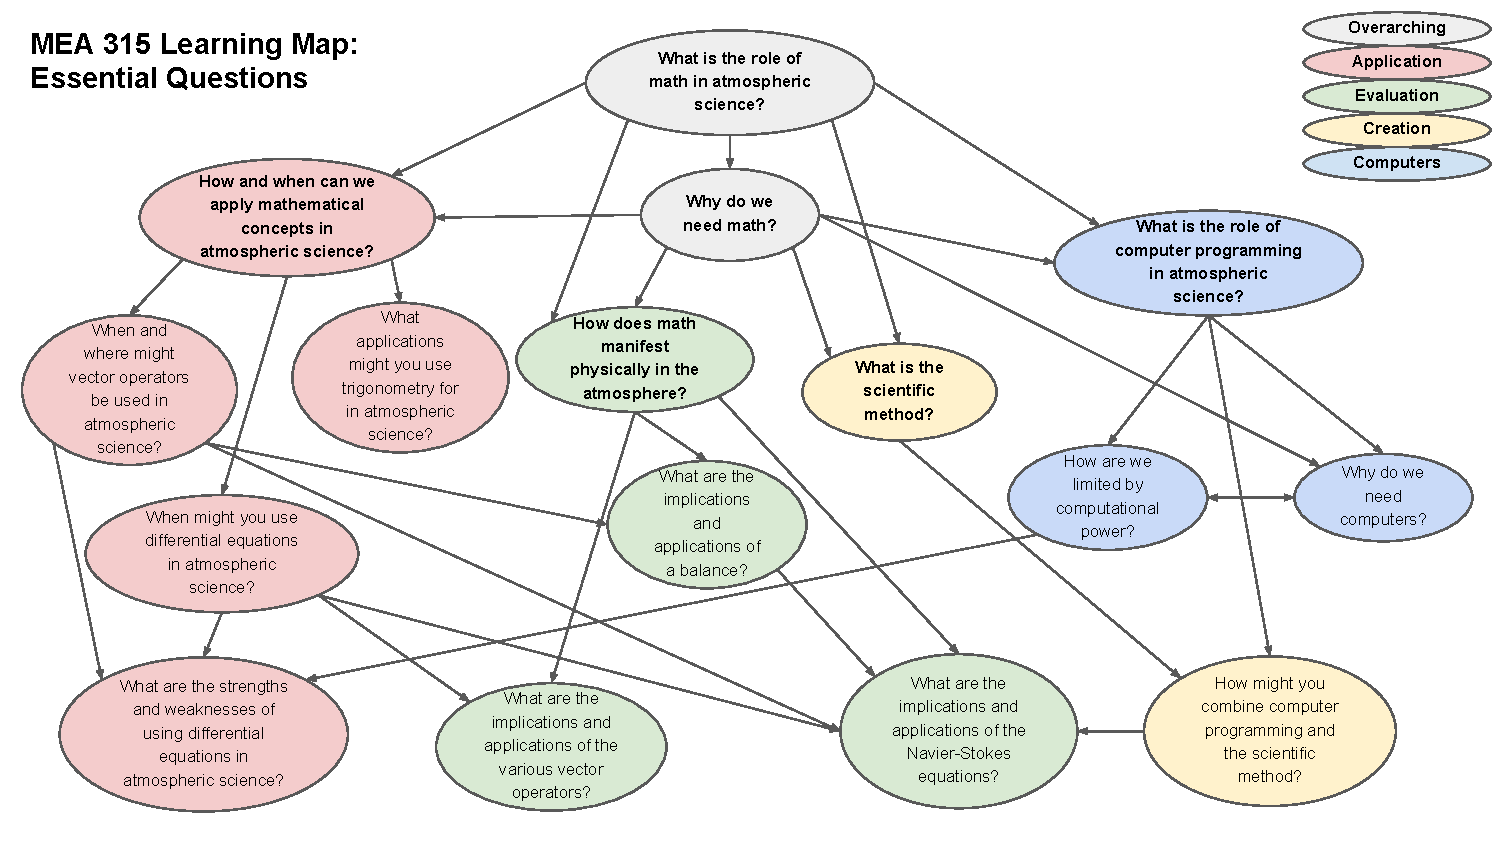
\includegraphics[width=1.3\textwidth,angle=90]{Concept_map_315.pdf}
% \end{figure*}

% Fifth Section %%%%%%%%%%%%%%%%%%%%%%%%%%%%%%%%%%%%%%%%%%%

\newpage
\section*{Course Policies}

\subsection*{During Class}
\footnotesize{I understand that the electronic recording of notes will be important for class and so computers will be allowed in class. Please refrain from using computers for anything but activities related to the class. Phones are prohibited as they are rarely useful for anything in the course. Eating and drinking are allowed in class but please refrain from it affecting the course. Try not to eat your lunch in class as the classes are typically active.}

\subsection*{Attendance Policy}
\footnotesize{For complete attendance and excused absence policies, please see http://policies.ncsu.edu/regulation/reg-02-20-03. Attendance is expected in all lecture and lab sections. Valid excuses for absence will be accepted before class. In extenuating circumstances, valid excuses with proof will be accepted after class. For every class missed the participation grade will be dropped 1 point.}

\subsection*{Policies on Incomplete Grades and Late Assignments}
\footnotesize{If an extended deadline is not authorized by the instructor or department, an unfinished incomplete grade will automatically change to an F after either (a) the end of the next regular semester in which the student is enrolled (not including summer sessions), or (b) the end of 12 months if the student is not enrolled, whichever is shorter. Incompletes that change to F will count as an attempted course on transcripts. The burden of fulfilling an incomplete grade is the responsibility of the student. The university policy on incomplete grades is located at http://policies.ncsu.edu/regulation/reg-02-50-3.}

\footnotesize{Late assignments will be accepted for no penalty if a valid excuse is communicated to the instructor before the deadline. After the deadline, assignments will be accepted for a 50\% deduction to the score up to 2 days after the deadline. After this any assignments handed in will be given 0.}

\subsection*{Academic Integrity and Honesty}
\footnotesize{Students are required to comply with the university policy on academic integrity found in the Code of Student Conduct found at http://policies.ncsu.edu/policy/pol-11-35-01. Don't cheat. Don't be that guy. Yes, you. You know exactly what I'm talking about. See http://policies.ncsu.edu/policy/pol-11-35-01 for a detailed explanation of academic honesty.}

\subsection*{Accommodations for Disabilities}
\footnotesize{Reasonable accommodations will be made for students with verifiable disabilities. In order to take advantage of available accommodations, students must register with the Disability Services Office at Suite 2221, Student Health Center, Campus Box 7509, 919-515-7653. For more information on NC State's policy on working with students with disabilities, please see the Academic Accommodations for Students with Disabilities Regulation (REG02.20.01) (https://policies.ncsu.edu/regulation/reg-02-20-01/).
Non-Discrimination Policy NC State University provides equality of opportunity in education and employment for all students and employees. Accordingly, NC State affirms its commitment to maintain a work environment for all employees and an academic environment for all students that is free from all forms of discrimination.}

\footnotesize{Discrimination based on race, color, religion, creed, sex, national origin, age, disability, veteran status, or sexual orientation is a violation of state and federal law and/or NC State University policy and will not be tolerated. Harassment of any person (either in the form of quid pro quo or creation of a hostile environment) based on race, color, religion, creed, sex, national origin, age, disability, veteran status, or sexual orientation also is a violation of state and federal law and/or NC State University policy and will not be tolerated. Retaliation against any person who complains about discrimination is also prohibited. NC State's policies and regulations covering discrimination, harassment, and retaliation may be accessed at \href{http://policies.ncsu.edu/policy/pol-04-25-05} or  \href{http://www.ncsu.edu/equal_op/}. Any person who feels that he or she has been the subject of prohibited discrimination, harassment, or retaliation should contact the Office for Equal Opportunity (OEO) at 919-515-3148.}